\documentclass[12pt,table,xcolor={dvipsnames}]{beamer}
\usetheme{Pittsburgh}
\usecolortheme{seagull}
%\usepackage[utf8]{inputenc}
\usepackage{fontspec}
\usepackage{amsmath}
\usepackage{listings}
\usepackage{multirow}
\usepackage{amsfonts}
\usepackage{amssymb}
\usepackage{graphicx}
\author{Design and Verification of Security Protocols and Security Ceremonies}
\title{\vspace{-1.2cm}Symmetric and Asymmetric Cryptographic \\\vspace{1.2cm} Primitives}
%\setbeamercovered{transparent} 
\setbeamertemplate{navigation symbols}{} 
%\logo{
\includegraphics[scale=0.015]{Brasao_UFSC.png}
\includegraphics[scale=0.2]{brasao_PPGCC.jpg}} 
\institute{Programa de Pós-Graduacão em Ciências da Computacão \\ Dr. Jean Everson Martina} 
\date{\vspace{.2cm}March-June 2019}  
\subject{} 
\usebackgroundtemplate{
\includegraphics[width=\paperwidth,
height=\paperheight]{../reusable_images/fundo_UFSC.png}}
\begin{document}

{
\usebackgroundtemplate{
\includegraphics[width=\paperwidth,
height=\paperheight]{../reusable_images/fundo_capa.png}}
\begin{frame}
\titlepage

\includegraphics[scale=0.3]{../reusable_images/brasao_PPGCC.jpg}
\end{frame}
}

\begin{frame}{Cryptography Aims}
\begin{columns}
\column{.5\textwidth}
\begin{itemize}
\item To provide confidentiality;\pause
\item Securely exchange information in an insecure environment;\pause
\item Only valid users know how to perform decryption.\pause
\end{itemize}
\column{.5\textwidth}
\begin{center}
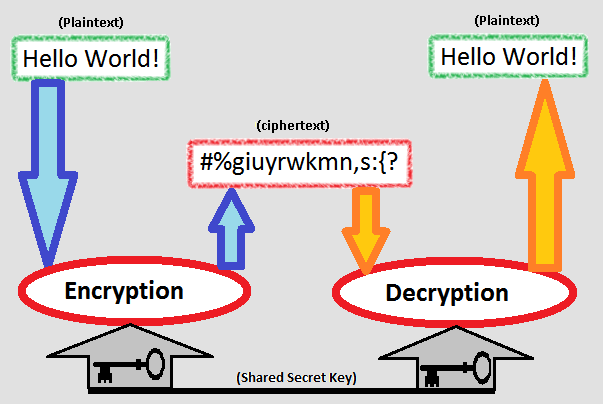
\includegraphics[scale=.35]{crypto.png}
\end{center}
\end{columns}
\end{frame}


\begin{frame}{Symmetric Cryptography Setting}
\begin{itemize}
\item Encryption and Decryption are specified algorithms;\pause
\item Two approaches:\pause
\begin{itemize}
\item Keep encryption and decryption algorithms secret: \textit{''security through
obscurity"};\pause
\item Add another variable, called a \textit{key} that must be known to encrypt and
decrypt a message;\pause
\end{itemize}
\item Symmetric-key cryptography uses same key used for both encryption and decryption.
\end{itemize}
\end{frame}


\begin{frame}{Symmetric Cryptography Problem}
\begin{itemize}
\item Symmetric-key cryptography requires that the recipient of an encrypted message knows the key;\pause
\item We can not send key in a separate message because:\pause
\begin{itemize}
\item If unencrypted an adversary could intercept it and learn the key;\pause
\item If encrypted it would require a key that had to be distributed somehow;\pause
\end{itemize} 
\item We usually assume the key is known;\pause
\item We will talk about key distribution protocols in the next lectures.
\end{itemize}
\end{frame}

\begin{frame}{Classical Cryptography}
\begin{itemize}
\item As remote as Julius Ceasar in ancient Rome or Sparta in ancient Greece;\pause
\item Substitution cipher: replace individual characters with different characters;\pause
\item Permutation cipher: change the order of the characters using permutations;\pause
\item Good modern symmetric ciphers use substitution and permutation;\pause
\item Its been the study of military schools for a long time;\pause
\item Developed the area of Cryptanalysis.
\end{itemize}
\end{frame}

\begin{frame}{Mono-alphabetic Ciphers}
\begin{itemize}
\item Same encryption algorithm used for each character;\pause
\item Problems are that:\pause
\begin{itemize}
\item Characters and words do not have enough entropy;\pause
\item Context defines how characters are used and when they are used;\pause
\end{itemize}
\item You attack such ciphers by measuring the distribution on cipher-text and comparing it with a target language;\pause
\item It can be made more efficient by using context of doubles and triples.
\end{itemize}
\end{frame}

\begin{frame}{Poly-alphabetic  Ciphers}
\begin{itemize}
\item Change the substitution pattern on a character-by-character basis;\pause
\item Uses a key to configure the selection of various mono-alphabetic ciphers;\pause
\item We can not apply frequency analysis directly because the translations scheme changes every new character we input;\pause
\item You attack if the user reuses the key throughout the encryption process;\pause
\item You find the period of the key and them use frequency analysis to crack all the mono alphabetic cipher independently.
\end{itemize}
\end{frame}

\begin{frame}{Electro-Mechanical Ciphers}
\begin{itemize}
\item The enigma machine challenged the boundaries of computable functions;\pause
\item It is a machine to assist the usage of poly-alphabetic ciphers;\pause
\item Every time a key is pressed rotors turn to change the substitution pattern;\pause
\item The problems the led to Enigma being cracked are:\pause
\begin{itemize}
\item Characters never mapped to themselves;\pause
\item E() = D();\pause
\item Operator errors;\pause
\item Known plain-text;\pause
\end{itemize}
\end{itemize}
\end{frame}


\begin{frame}{Shannon's  Information Theory}
\begin{itemize}
\item In 1948, Claude Shannon invented the basis of Information Theory in his publication ``A Mathematical Theory of Communication;\pause
\item Provably secure means the key must be just as random as the cipher-text;\pause
\item This would lead to an infinite number of possible meaningful decryption;\pause
\item One-Time Pad can be implemented with Viginere or XOR;\pause
\item Provably secure if you do not reuse the key;
\end{itemize}
\end{frame}


\begin{frame}{Stream Ciphers How-To}
\begin{itemize}
\item Start with a secret key to seed a generator;\pause
\item Generate a keying stream that do not repeat itself;\pause
\item The i-th bit of keying stream is a function of the key and the first i-1 cipher-text bits;\pause
\item Combine the stream with the plain-text to produce the cipher-text (typically by XOR);\pause
\item Revert it by applying the key-stream again.
\end{itemize}
\end{frame}

\begin{frame}{Stream Ciphers Implementations}
\begin{itemize}
\item Most pre computer tools used stream ciphers;\pause
\item The German Enigma machine;\pause
\item Linear Feedback Shift Register;\pause
\item A5 – encrypting GSM handset to base station communication;\pause
\item RC-4 (Ron’s Code) WEP Encryption.
\end{itemize}
\end{frame}

\begin{frame}{Stream Ciphers Implementations}
\begin{itemize}
\item Advantages:\pause
\begin{itemize}
\item Speed of transformation: algorithms are linear in time and constant in space;\pause
\item Low error propagation: an error in encrypting one symbol Likely will not affect subsequent symbols;\pause
\end{itemize}
\item Disadvantages:\pause
\begin{itemize}
\item Low diffusion: all information of a plain-text symbol is contained in a single cipher-text symbol;\pause
\item Susceptibility to insertions/ modifications: an active interceptor who breaks the algorithm might insert spurious text that looks authentic.
\end{itemize}
\end{itemize}
\end{frame}

\begin{frame}{Block Ciphers}
\begin{itemize}
\item Encrypt a block of input to a block of output;\pause
\item Typically, the two blocks are of the same length;\pause
\item Symmetric key systems block size vary from 64 to 256 bits;\pause
\item Has different modes for encrypting plain-text longer than a block and this affects security.
\end{itemize}
\end{frame}

\begin{frame}{Block Ciphers Implementations}
\begin{itemize}
\item DES, 3-DES;\pause
\item AES;\pause
\item RC-2, RC-5;\pause
\item IDEA;\pause
\item Blowfish, Twofish;\pause
\end{itemize}
\end{frame}

\begin{frame}{Block Ciphers Implementations}
\begin{itemize}
\item Advantages:\pause
\begin{itemize}
\item High diffusion: information from one plain-text symbol is diffused into several cipher-text symbols;\pause
\item Immunity to tampering: difficult to insert symbols without detection;\pause
\end{itemize}
\item Disadvantages:\pause
\begin{itemize}
\item Slowness of encryption: an entire block must be accumulated before encryption/decryption can begin;\pause
\item Error propagation: An error in one symbol may corrupt the entire block.
\end{itemize}
\end{itemize}
\end{frame}

\begin{frame}{ECB Mode of Encryption}
\begin{columns}
\column{.5\textwidth}
\begin{itemize}
\item Simple and efficient;\pause
\item Parallel implementation possible;\pause
\item Does not conceal plain-text patterns;\pause
\item Active attacks are possible.\pause
\end{itemize}
\column{.5\textwidth}
\begin{center}
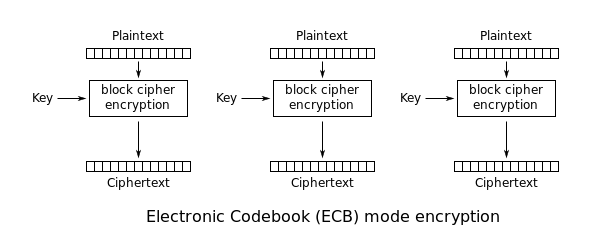
\includegraphics[scale=.25]{ECB_encryption.png}\pause\\
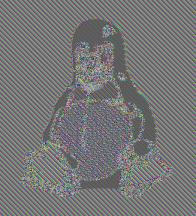
\includegraphics[scale=.35]{Tux_ecb.jpg}
\end{center}
\end{columns}
\end{frame}

\begin{frame}{CBC Mode of Encryption}
\begin{columns}
\column{.5\textwidth}
\begin{itemize}
\item It is an asynchronous stream cipher;\pause
\item Errors in one cipher-text block propagate to other blocks;\pause
\item Conceals plain-text patterns into cypher-text;\pause
\item Parallel implementation not known;\pause
\item It is difficult to manipulated Plain-text.
\end{itemize}
\column{.5\textwidth}
\begin{center}
\includegraphics[scale=.25]{CBC_encryption.png}\pause\\

\includegraphics[scale=.35]{Tux_secure.jpg}
\end{center}
\end{columns}
\end{frame}

\begin{frame}{OFB Mode of Encryption}
\begin{columns}
\column{.5\textwidth}
\begin{itemize}
\item It is an asynchronous stream cipher;\pause
\item Errors in one cipher-text block propagate to other blocks;\pause
\item Pre-processing is possible;\pause
\item Conceals plain-text patterns into cypher-text;\pause
\item Parallel implementation not known;\pause
\item Active attacks are possible.\pause
\end{itemize}
\column{.5\textwidth}
\begin{center}
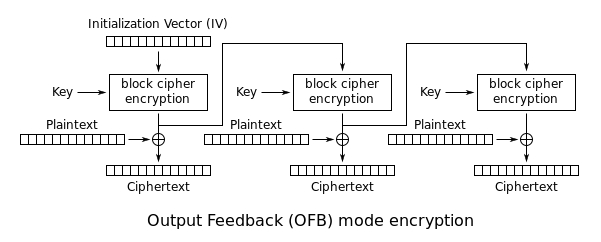
\includegraphics[scale=.25]{OFB_encryption.png}\pause\\

\includegraphics[scale=.35]{Tux_secure.jpg}
\end{center}
\end{columns}
\end{frame}

\begin{frame}{Hash Function}
\begin{itemize}
\item Length-reducing function h;\pause
\item Maps an arbitrary string to a fixed-length string;\pause
\item Publicly known;\pause
\item Also known as cryptographic checksums or message digests;\pause
\end{itemize}
\end{frame}

\begin{frame}{Hash Properties}
\begin{itemize}
\item Ease of computation;\pause
\item Pre-image resistance Collision;\pause
\item Collision;\pause
\item 2nd pre-image resistance;\pause
\item Collision resistance;\\\pause
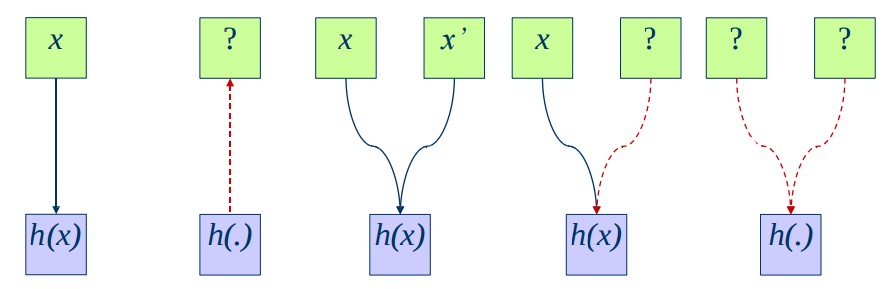
\includegraphics[scale=.3]{hash_properties.png}
\end{itemize}
\end{frame}

\begin{frame}{Message Authentication Codes}
\begin{itemize}
\item They couple the idea of an integrity checking functions with shared key crypto-system;\pause
\item They are also length reducing functions;\pause
\item They are publicly known;\pause
\item And ease of computation.
\end{itemize}
\end{frame}

\begin{frame}{MAC Functions' Properties}
\begin{itemize}
\item Given $n$ pairs $(m_1, MAC_k(m_1))$,..., $(m_n, MAC_k(m_n))$ find a new  pair $(m, MAC_k(m))$ efficiently and with non negligible probability is unlikely;\pause
\item Output should be a length-reduction function;\pause
\item The key should control the mapping between the Domain and Image of the MAC function, but not determine its spread.
\end{itemize}
\end{frame}

\begin{frame}{MAC Construction}
\begin{itemize}
\item There are basically two mains ways of producing secure MAC systems:\pause
\begin{itemize}
\item Symmetric CBC-MAC;\pause
\item CMAC;\pause
\item Hash based HMAC;
\end{itemize}
\end{itemize}
\end{frame}

\begin{frame}{CBC-MAC Mode of Encryption}
\begin{columns}
\column{.5\textwidth}
\begin{center}
\includegraphics[scale=.25]{../Lecture_2/CBC_encryption.png};
\end{center}
\column{.5\textwidth}
\begin{itemize}
\item It is basically the application of CBC over input data;\pause
\item Instead of keeping all the blocks we just keep the last one;\pause
\item Its length is determined by block size;\pause
\item IV is fixed.
\end{itemize}
\end{columns}
\end{frame}

\begin{frame}{Security of CBC-MAC}
\begin{itemize}
\item Secure for messages of a fixed number of blocks assuming the block cipher is Pseudo-Random Permutation;\pause
\item Not secure with variable lengths;\pause
\item Needs to be used with one key to each message length or do length pre-pending;
\end{itemize}
\end{frame}

\begin{frame}{CMAC}
\begin{columns}
\column{.5\textwidth}
\begin{center}
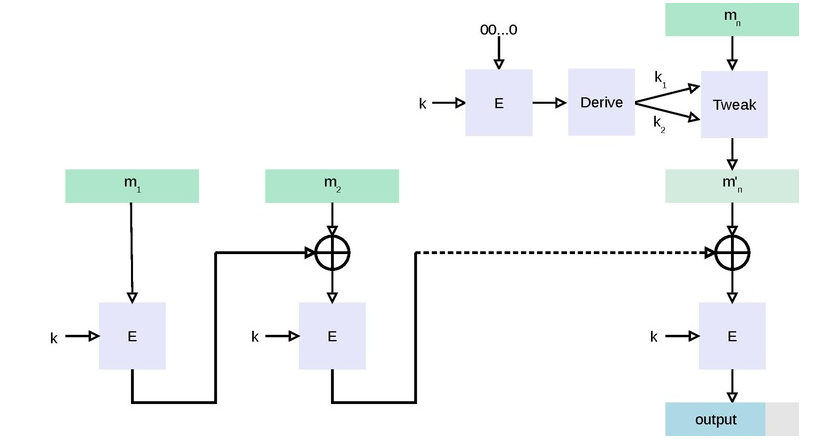
\includegraphics[scale=.22]{OMAC.png}
\end{center}
\column{.5\textwidth}
\begin{itemize}
\item It is a NIST standard for doing MAC with symmetric cyphers;\pause
\item Efficiently addresses the security deficiencies of CBC-MAC;\pause
\item Derives 2 keys to cypher the last block;
\end{itemize}
\end{columns}
\end{frame}

\begin{frame}{HMAC Properties}
\begin{itemize}
\item Use available hash functions without modification;\pause
\item Preserve the original performance of the hash function;\pause
\item Use and handle keys in a simple way;\pause
\item Allow easy replacement of the underlying hash function;\pause
\item Have a well-understood analysis of the strength of the authentication mechanisms;
\end{itemize}
\end{frame}

\begin{frame}{HMAC}
\begin{center}
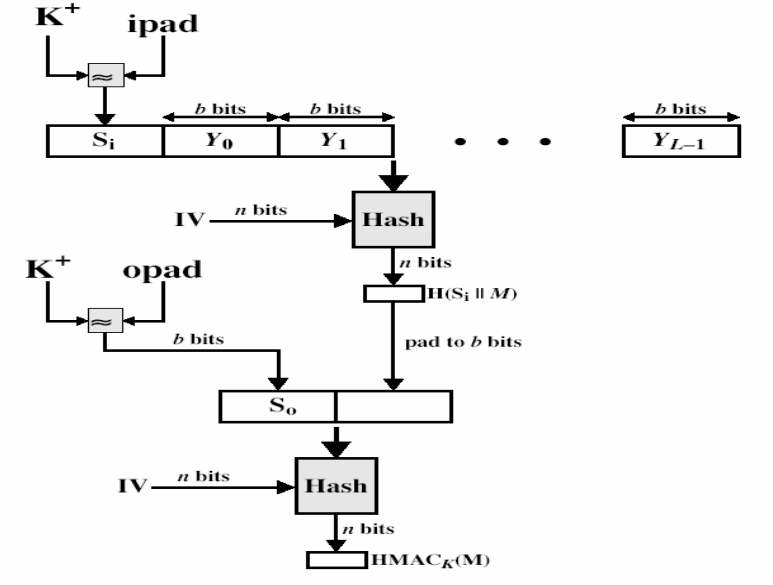
\includegraphics[scale=.33]{HMAC.png}
\end{center}
\end{frame}

\begin{frame}{Security of HMAC}
\begin{itemize}
\item Security of HMAC relates to that of the underlying hash algorithm;
\item If used with a secure hash functions and according to the specification (key size, and use correct output), no known practical attacks;
\end{itemize}
\end{frame}

\begin{frame}{Properties of Symmetric Encryption}
\begin{itemize}
\item Confidentiality of course!!!
\item How to achieve authentication?
\item And timeliness?
\item And Integrity
\end{itemize}
\end{frame}

\begin{frame}{Asymmetric Cryptography}
\begin{itemize}
\item Appeared on the 1970s. First classified by GCHQ and later publicly by Diffie and Helmann's work;\pause
\item Comes to solve the secure distribution channel on symmetric cryptography;\pause
\item A user has two keys: a public key and a private key;\pause 
\item Usually it is thousand of times more computationally intensive than symmetric cryptography.
\end{itemize}
\end{frame}

\begin{frame}{Asymmetric Crypto-system Properties}
\begin{itemize}
\item A message can be encrypted with the public key and decrypted with the private key to provide security;\pause
\item A message can be encrypted with the private key and decrypted with the public key to provide signatures;\pause
\item Security is related to strong mathematical problems;\pause
\item Usually these problems are both polynomial time, but there can be a trapdoor to solve it quickly;\pause
\item A lot of theoretical work compared to symmetric cryptography;\pause
\item Usually based on finite fields constrained by modular operations.\pause
\end{itemize}
\end{frame}

\begin{frame}{Private Keys}
\begin{itemize}
\item There is a strong assumption on its possession;\pause
\item Properties yielded are related to its owners executing their will;\pause
\item Strong mathematical relation between itself and its public counterpart;\pause
\item Finding it by random should be possible but with negligible probability;\pause
\item Derive it either from cypher-text and from public key should not be possible;\pause
\item Provides authentication but does not provide confidentiality.
\end{itemize}
\end{frame}

\begin{frame}{Public Keys}
\begin{itemize}
\item There is a strong assumption on relation to identity;\pause
\item Properties yielded are related to its other verifying the owners will;\pause
\item Strong mathematical relation between itself and it private counterpart;\pause
\item It should be as public as possible;\pause
\item Does not provide authentication but only confidentiality.
\end{itemize}
\end{frame}

\begin{frame}{Key Space}
\begin{itemize}
\item Way bigger than symmetric cryptography;\pause
\item Usually this happens because not everything can be a key;\pause
\item To operate with all mathematical properties the filed should be constructed over the idea of primality;\pause
\item Primality can be defined in different ways for different fields;\pause
\item Modular Exponentiation and Discrete Logarithm are the problems;\pause
\item Keys are defined for these operations.
\end{itemize}
\end{frame}

\begin{frame}{Digital Signatures Mode}
\begin{itemize}
\item Yields Authenticity of messages;\pause
\item Desirable properties of a digital signature:\pause
\begin{itemize}
\item A receiver must be able to validate the signature;\pause
\item The signature must not be forgeable; \pause
\item The signer must not be able to repudiate the signature;\pause
\end{itemize}
\item Encrypt with private key, validate with public key;\pause
\item For security and authenticity, encrypt the signed message with the receiver’s public key;
\end{itemize}
\end{frame}

\begin{frame}{Encryption Mode}
\begin{itemize}
\item Yields Confidentiality of messages;\pause
\item Guarantees the intended destination of a message;\pause
\item Strongly related to the possession of the private key;\pause
\item Usually has problems with messages bigger than key sizes;\pause
\end{itemize}
\end{frame}

\begin{frame}{Example of Asymmetric Algorithms}
\begin{itemize}
\item Diffie–Hellman;\pause
\item DSS (Digital Signature Standard);\pause
\item ElGamal;\pause
\item RSA encryption algorithm (PKCS\#1);\pause
\item Cramer–Shoup cryptosystem;\pause
\item etc...
\end{itemize}
\end{frame}

\begin{frame}{The Protocol's Questions?}
\begin{itemize}
\item How to achieve our goals consuming less computational power?\pause
\item How do we overcome algorithms shortcomings? \pause
\item How do we change the properties to achieve less or more?\pause
\item How can we achieve properties other than the yielded by algorithms?\pause
\item How can I be sure of what I did?
\end{itemize}
\end{frame}


{
\usebackgroundtemplate{
\includegraphics[width=\paperwidth,
height=\paperheight]{../reusable_images/fundo_capa.png}}
\begin{frame}

{\LARGE Questions????}

\end{frame}
}

{
\usebackgroundtemplate{
\includegraphics[width=\paperwidth,
height=\paperheight]{../reusable_images/fundo_capa.png}}
\begin{frame}

\includegraphics[scale=0.8]{../reusable_images/cc_logo_arge.png}\hspace{0.5cm} 

\includegraphics[scale=0.95]{../reusable_images/by.png}

\vspace{1cm}
This work is licensed under the Creative Commons Attribution 4.0 International License. To view a copy of this license, visit http://creativecommons.org/licenses/by/4.0/.
\end{frame}
}

\end{document}
